%
% File: chap01.tex
% Author: Liam O'Shea
% Description: Introduction chapter where the boxing goes.
%
\let\textcircled=\pgftextcircled
\chapter{Specification \& Design}
\label{chap:intro}

\initial{T}his needs to give a general overview of the program structure/system architecture.


%=======
\section{Scope of Project}
\label{sec:sec01}
Begins a section.

\section{Punch Segmentation Algorithm}

\section{Punch Quality Algorithm}
I will be measuring quality in reference to a `ground truth' produced by a local professional. My aim is to create rules that are capable of detecting basic mistakes and offer advice accordingly. 
Jab sticking the right elbow up.



\section{Segmentation methods? Feature Extraction?}


\subsection{Dynamic Time Warping (DTW)}
Dynamic time warping compares two temporal sequences, often which vary in time or speed and tries to calculate an optimal match. The two sequences are aligned and a similarity score is produced. This technique can be used on any data that can be represented in a linear fashion and has been successfully applied to fields such as signature recognition, voice recognition, partial shape matching and gait analysis. For example in gait analysis, similarities could be detected in the walking pattern of two people even though their speed and acceleration may be difference. 
\textcolor{red}{Given I will be measuring punches of sequences over time I intend to see If I can use DTM to recognise punches and pose}


\subsection{Neural Networks}
Neural networks are models based on the parallel processing of information similar to that of the brain. A NN can be configured for different applications such as clustering, pattern recognition, Dynamic Time series and curve fitting. They are able to derive meaning from complex data that human beings would be unable to notice and that other techniques will fail on. Crucially the networks are capable of approximating non-linear functions \textbf{unlike DTW. Neural networks learn by examples in the form of training data and are adaptive based on a system of weightings calculated by \% error.Other characteristics are their ability to self organise and the ability to work in real-time if sufficient parallelism is supported.}


\subsection{Decision Trees}
A predictive tree like model which maps observations about an object to reach a conclusion about its target value. In this model the `leaves' represent class labels while the branches themselves represent conjunctions of features that will lead to the class labels. Put simply each condition in an internal node while each outcome is an external node. 
{H = – SUM_OF_ALL_THE_EVENTS(the probability of the event * log2(the probability of the event}

Information gain is the difference between the initial entropy and the new entropy after following a branch along the decision tree. Since the goal in machine learning is to achieve a low value of entropy to make accurate predictions, the decision tree is constructed such that each branch has the maximum possible information gain. The data is split by each feature that has the maximum information gain recursively for each branch.



\begin{figure}[h]
    \centering
    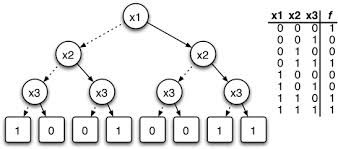
\includegraphics[height=0.25\textheight]{fig03/dtree}
    \mycaption[Kinect Device]{Kinect Device.}
    \label{fig:kinect}
\end{figure}


\subsection{Support Vector Machines}
A Support Vector Machine is a, kernel-based method that is effective for high 
dimensional datasets. The SVM uses a kernel to calculate the scalar product of two feature vectors in a high dimensional feature space. The decision function uses the hyper-planes, defined by the Support  vectors,  to  classify  the  data.  Only  significant  samples  are  taken  for  use  as support vectors so that a high variance will make less of a different to the accuracy of the model. {This is well suited to a recognition task as the same punches will be thrown slightly differently.}

\begin{figure}[h]
    \centering
    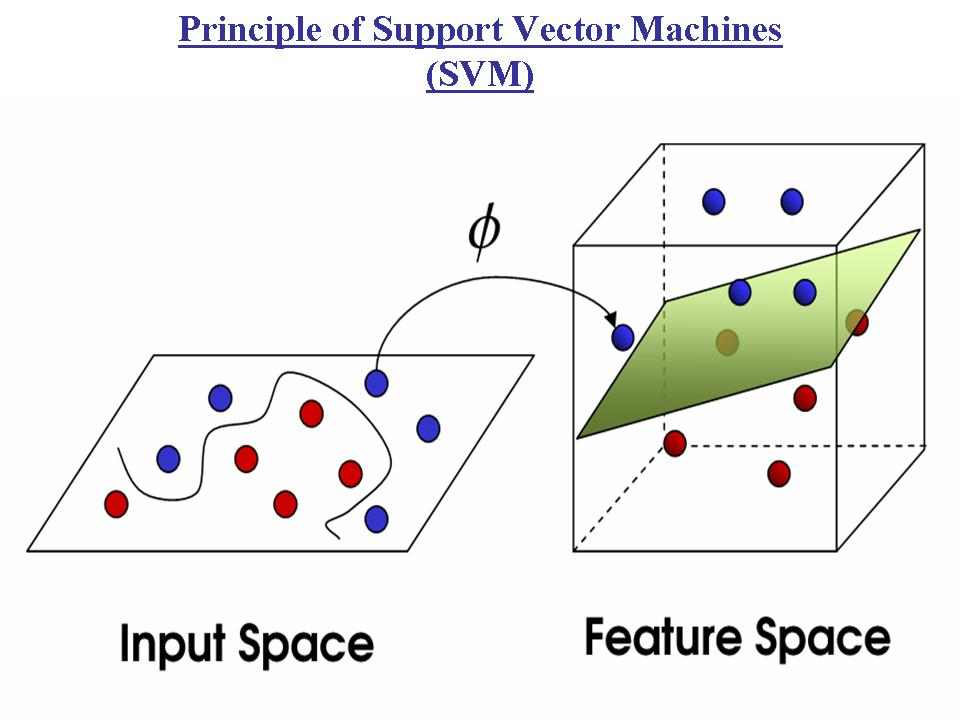
\includegraphics[height=0.25\textheight]{fig03/svm}
    \mycaption[Kinect Device]{Kinect Device.}
    \label{fig:kinect}
\end{figure}

\subsection{Fourier Transformation}

The FT is a mathematical transformation that transforms signals from the spatial domain (normal image space) into the frequency domain. It allows a signal to be split in a phase and magnitude spectrum.

Since my punches are a continuous periodic function over time, the Fourier transformation can be simplified to a set of complex amplitudes know as Fourier Series Coefficients. These represent the frequency domain of the original signal and can be used to recreate the signal if required. {\bf I DO THIS}



{How did I use it? What is the significance in the coefficient difference between certain punches? Why does the right hand have a higher coefficient?}
\textcolor{red}{Figure of FFT?}


\section{Dimensionality}
\paragraph{Curse of Dimensionality}
The curse of dimensionality, first discussed by Richard E Bellman in his book Dynamic Programming\cite{dynprog} is the term for a set of problems that occur when using high dimensionality data. As dimensionality increases as does the search space, resulting in the available data become sparse. In order to obtain accurate, reliable and statistically sound results the total amount of data required can grow exponentially in relation to the dimensionality. Likewise the organisation and searching of non-reduced data becomes difficult, {\bf with space and search time dependent on data volume.} Searching and organising data also relies on the ability to group instances into groups that share similar characteristics, unfortunately if the data appears to be dissimilar due to sparseness it can prevent {\bf grouping strategies} 

Algorithms that can successfully deal with high dimensionality data typically will have high time complexity and {\bf will not always} produce more accurate results than algorithms that work on the lower dimensionality data. Therefore it is sensible to look at some dimensionality reduction techniques which {\bf might} produce better results.

Furthermore since the long-term goal is to give feedback with live data, speed is of the essence. Therefore dimensionality reduction is an important component required to decrease the processing time on any input.

\subsection{Dimensionality Reduction}
Dimensionality Reduction is the process of reducing the number of variables under consideration for any given problem. For example each frame from the Kinect is represented as 60 features, the x,y,z co-ordinates of the 20 skeleton joints. Considering the Kinect is capable of 30 FPS that is $1800$ data points per second of movement. {\bf With long sequences of recordings this could become a huge amount of data, most of it not actually relevant to the specific features we are looking for. As a result Dimensionality reduction seems like a sensible path.}

\subsection{Principal Component Analysis (PCA)}
\label{subsec:subsec01}
Principal Component Analysis is a statistical procedure that transformed a set of observations of potentially correlated variables into a set of linearly uncorrelated variables called principal components. The number of principal components should always be less than or equal to the number of original values with the first principal component having the largest possible variance. Each following component will attempt to represent as much variance in the data as possible. In my case I will be looking to reduce my 60 data points per frame into a low dimensionality set that will help me to uniquely identify punches.


\section{Manifold Learning}
Manifold learning is a Non-Linear Dimensionality Reduction process that transforms high dimensionality data that typically requires multiple dimension to represent it which is difficult to interpret. To simplify the data it is possible to assume that the date lies on an embedded non-linear manifold within the high-dimensionality space. Assuming the manifold has low enough dimensions it can then be visualised in this lower-dimensionality space.

\subsection{Markov Chains}
Markov chains are a series of `states' which have a probability for each transition and are used to model real world events.

\begin{figure}[h]
    \centering
    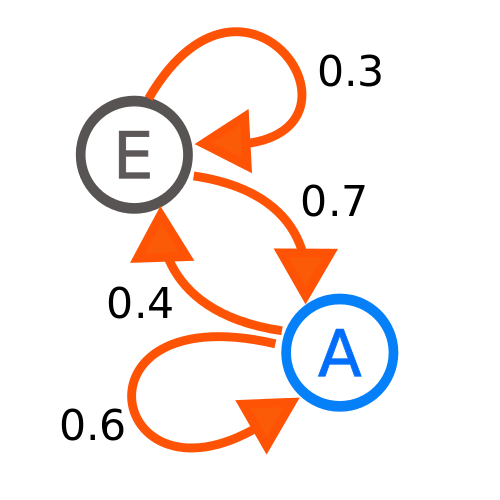
\includegraphics[height=0.25\textheight]{fig03/markov}
    \mycaption[Kinect Device]{Kinect Device.}
    \label{fig:kinect}
\end{figure}




\subsection{Diffusion Maps}
Diffusion maps are a non-linear and relatively new technique developed in 2006 by Ronald R. Coifman and Stephane Lafon.\cite{Coifman2006} The aim of a diffusion map is to provide a framework for finding meaningful geometric descriptions of data sets. Diffusion maps are capable of turning high dimensionality data into low dimensional structure. Unlike other dimensionality reduction techniques like PCA, diffusion maps attempt to discover the underlying manifold, a lower dimensional constrained surface containing the data.Diffusion maps are based on defing a Markov random walk on the graph of the data. By performing this for a set number of time steps a measure for the proximity of datapoints is obtained, which is used to define a diffusion distance. Pairwise diffusion distance are retained as well as possible in the dimensionally reduced data.


\textcolor{red}{Figure of diffusion map}


\subsection{Locally Linear Embedding (LLE)}
In LLE a data manifold is constructed by finding a set of the nearest neighbours for each point. Together they are used to compute a set of weights that describes each point as a linear combination of its neighbours.
Finally, it uses an eigenvector-based technique to find the low-dimensional embedding of points, such that each point is still described with the same linear combination of its neighbours. Furthermore, the preservation of local properties allows for successful embedding of non convex manifolds.
{\bf LLE tends to handle non-uniform sample densities poorly because there is no fixed unit to prevent the weights from drifting as various regions differ in sample densities.}




\subsection{Laplacian Eigenmaps}\cite{Belkin2003}
Laplacian Eigenmaps find a low-dimensional data representation by preserving local properties of the
manifold. Similar to LLE, a graph is built from neighbourhood information, with the distance between a point and it's K nearest neighbour is minimised. A weighting system is used such that in the low-dimensionality space the distance from a point to it's nearest neighbour is more significant to the cost function than other nearby points. {\bf put simply the closer a neighbour is to the selected data point the heavier its weighting.} The goal overall is to minimise the cost function based on the graph information to ensure that points close together in the high dimensionality data remain so after the reduction, preserving local distances. 



\subsection{Local Tangent Space Alignment (LTSA)}
LTSA[30] is based on the intuition that when a manifold is correctly unfolded, all of the tangent hyperplanes to the manifold will become aligned. It begins by computing the k-nearest neighbours of every point. It computes the tangent space at every point by computing the d-first principal components in each local neighbourhood. It then optimizes to find an embedding that aligns the tangent spaces.

Similar to Hessian LLE, Local Tangent Space Analysis (LTSA) is a technique that describes local properties of the
high-dimensional data using the local tangent space of each datapoint [93]. LTSA is based on the observation that, if
local linearity of the manifold is assumed, there exists a linear mapping from a high-dimensional datapoint to its local
tangent space, and that there exists a linear mapping from the corresponding low-dimensional datapoint to the same
local tangent space [93]. LTSA attempts to align these linear mappings in such a way, that they construct the local
tangent space of the manifold from the low-dimensional representation. In other words, LTSA simultaneously searches
for the coordinates of the low-dimensional data representations, and for the linear mappings of the low-dimensional
datapoints to the local tangent space of the high-dimensional data





\subsection{Curvilinear Component Analysis (CCA)}

Similar to Hessian LLE, Local Tangent Space Analysis (LTSA) is a technique that describes local properties of the
high-dimensional data using the local tangent space of each datapoint [93]. LTSA is based on the observation that, if
local linearity of the manifold is assumed, there exists a linear mapping from a high-dimensional datapoint to its local
tangent space, and that there exists a linear mapping from the corresponding low-dimensional datapoint to the same
local tangent space [93]. LTSA attempts to align these linear mappings in such a way, that they construct the local
tangent space of the manifold from the low-dimensional representation. In other words, LTSA simultaneously searches
for the coordinates of the low-dimensional data representations, and for the linear mappings of the low-dimensional
datapoints to the local tangent space of the high-dimensional data

Curvilinear component analysis (CCA)[11] looks for the configuration of points in the output space that preserves original distances as much as possible while focusing on small distances in the output space (conversely to Sammon's mapping which focus on small distances in original space).
It should be noticed that CCA, as an iterative learning algorithm, actually starts with focus on large distances (like the Sammon algorithm), then gradually change focus to small distances. The small distance information will overwrite the large distance information, if compromises between the two have to be made.
The stress function of CCA is related to a sum of right Bregman divergences[12]




%=========================================================

Kinect pipeline?

